\documentclass[twocolumn]{article}
\usepackage[portuguese]{babel}
\usepackage[utf8]{inputenc}
\usepackage{amsmath}
\usepackage{subcaption}
\usepackage{mathtools}
\usepackage{graphicx}
\usepackage{color}
\usepackage{authblk}
\usepackage[colorlinks,citecolor=red,urlcolor=blue,bookmarks=false,hypertexnames=true]{hyperref}
\usepackage[top=15mm, bottom=15mm, left=15mm, right=15mm]{geometry}


\usepackage[alf, abnt-etal-list=0, abnt-emphasize=bf,abnt-last-names=bibtex, abnt-etal-text=it, abnt-etal-cite=2]{abntex2cite}

\title{Título}
\author{Leandro Vieira dos Santos}
\affil{EREM Regina Pacis\\Palmerina-PE}

\usepackage{lipsum}

\begin{document}

\maketitle        

\begin{abstract}
\lipsum[1]
s\end{abstract}


\section{Introdução}

\lipsum[1]

\section{Metodologia}

\lipsum[3]

\subsection{Título}\label{sec_titulo}

\lipsum[2]

\begin{figure}[!htb]
	\centering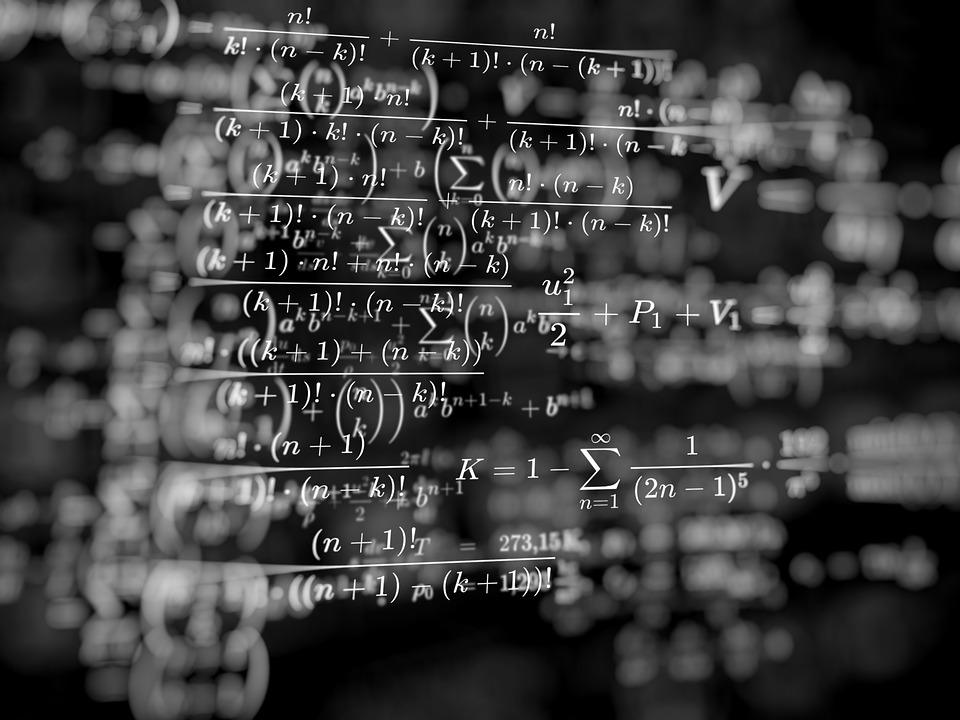
\includegraphics[width=\columnwidth]{Figuras/imagem}\\
	\caption{Imagem}\label{im}
\end{figure}

\lipsum[4]

\begin{figure}[!htb]
	\centering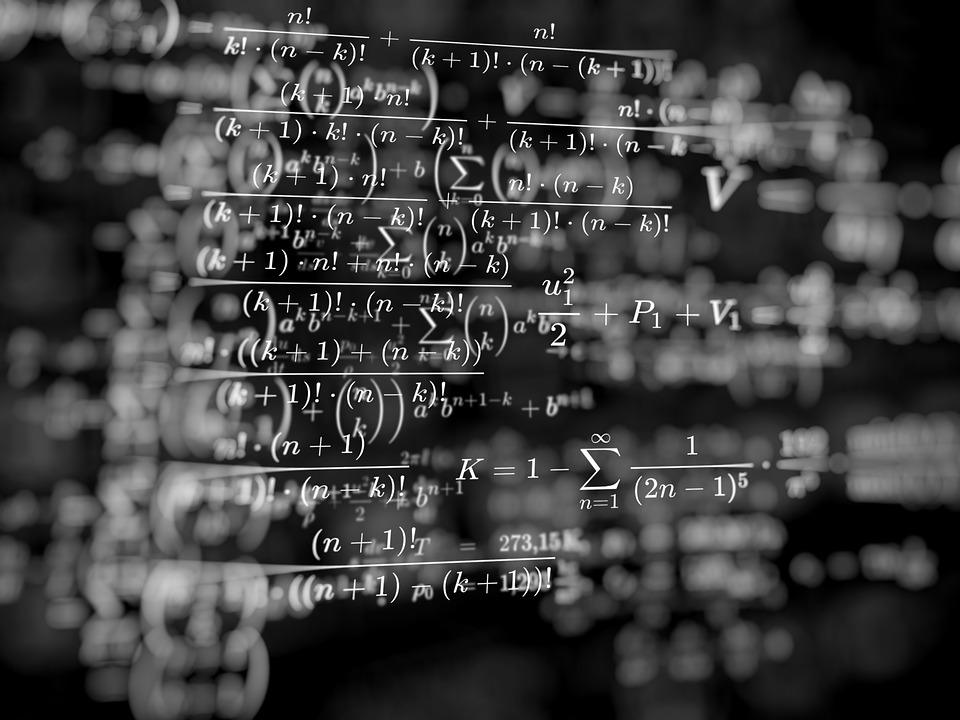
\includegraphics[width=\columnwidth]{Figuras/imagem}\\
	\caption{Imagem}\label{im}
\end{figure}

\lipsum[5]

\begin{figure}[!htb]
	\centering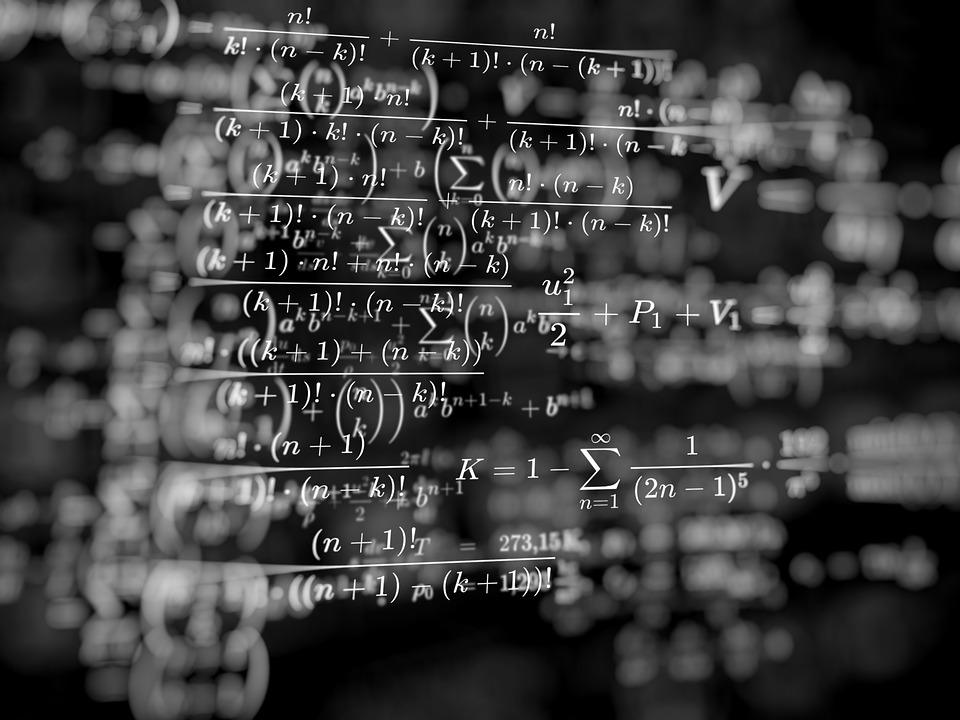
\includegraphics[width=\columnwidth]{Figuras/imagem}\\
	\caption{Conexão do motor trifásico em estrela. }\label{triangulo}
\end{figure}

Na \ref{sec_titulo} Acontece

\bibliography{refs}
\begin{thebibliography}{refs}
\bibitem{}

\end{thebibliography}
\end{document}